\documentclass[aspectratio=169, handout, 10pt, hyperref=colorlinks]{beamer}

\renewcommand\appendixname{Appendix}

\usetheme{Boadilla}

\title{Coded Compressed Sensing Scheme for
Unsourced Multiple Access}

\subtitle{CS754 Advanced Image Processing}

\author[Team CCS]{Rathour Param Jitendrakumar, 190070049 \texorpdfstring{\\} \ \and  Satush Parikh, 21D070062  }
% - Give the names in the same order as the appear in the paper.
% - Use the \inst{?} command only if the authors have different
%   affiliation.
\institute[IIT Bombay]{Indian Institute of Technology Bombay\\\url{https://github.com/paramrathour/Coded-Compressed-Sensing-for-Unsourced-Multiple-Access}}

\date{Spring 2023-24}

\subject{Coded Compressed Sensing}

\usepackage{braket}
\usepackage{epigraph}
\usepackage{fancyvrb}
\usepackage{amsmath,amssymb,amsfonts,mathtools,nccmath,bm}
\usepackage{algorithm}
% \usepackage[shortlabels]{enumitem}
\usepackage{algpseudocode}
\usepackage{graphicx}
\graphicspath{{images}}
\usepackage[aboveskip=-0.5em, belowskip=0em]{subcaption}
\usepackage{textcomp}
\usepackage{xcolor}
\usepackage{float}
\usepackage{tikz}
% \hypersetup{colorlinks, linkcolor=magenta}
\usepackage{ragged2e}
% \usepackage{etoolbox}
% \apptocmd{\frame}{}{\justifying}{} % Allow optional arguments after frame.
\renewcommand{\raggedright}{\leftskip=0pt \rightskip=0pt plus 0cm}
\apptocmd{\frame}{}{\justifying}{}
% \addtobeamertemplate{}{}{\justifying}
\setbeamersize{text margin left=2em,text margin right=3em}
% \setlength\abovecaptionskip{-5pt}
% \beamerdefaultoverlayspecification{<+->}
% \addtobeamertemplate{proof begin}{%
%     \setbeamercolor{block title}{fg=red!50!black,bg=red!25!white}%
%     \setbeamercolor{block body}{fg=black, bg=red!10!white}%
% }{}
% % \newcommand{\lenitem}[2][.7\linewidth]{\parbox[t]{#1}{\strut #2\strut}}

\newtheorem{defn}{Definition}
\newtheorem{lem}{Lemma}
\newtheorem{prop}{Proposition}
\theoremstyle{example}
\newtheorem{postulate}{Postulate}
\newtheorem{assumption}{Assumption}
% \newtheorem{problem}{Problem}
% \newtheorem{note}{Note}

\renewcommand{\d}{\, \mathrm{d}}
\newcommand{\R}{\ensuremath\mathbb{R}}
\newcommand{\op}[1]{\operatorname{#1}}


\begin{document}

\begin{frame}
  \titlepage
  \begin{center}
    Guide: Prof. Ajit Rajwade
  \end{center}
%   \epigraph{When you go to sleep make sure there is someone to wake you up.}{Prof. Mythili Vutukuru}
\end{frame}

\begin{frame}{Outline}
  \tableofcontents
  % You might wish to add the option [pausesections]
\end{frame}



\section{Introduction}
\subsection{Unsourced Multiple Access}
\begin{frame}{Implementation}{Unsourced Multiple Access}
\begin{itemize}
    \item Problem
    \begin{itemize}
        \item Transmitting messages to the access point in ann uncoordinated fashion
            \item All users employ a common codebook 
            \item  The receiver decodes up to a permutation of the messages
            % \begin{itemize}
            % \item RGB to Grayscale conversion
            % \item Normalisation of Image Sets
            % \end{itemize}
            \item Unsourced multiple access (UMAC) - the use of a unique code does not allow to distinguish the transmitters identity.
        \end{itemize}
     \item Assumption
     \begin{itemize}
         \item Active devices pick their information message independently and uniformly at random from the set of binary sequences $\{0,1\}^B.$
     \end{itemize}
\end{itemize}
\end{frame}

\begin{frame}{System Model}
\begin{itemize}
    \item  $\mathbf{S}_{\mathrm{a}}$$\subset\mathbf{S}_{\mathrm{tot}}$ - collection of devices within a network (Cardinality $K_{\mathrm{tot}}$)
    \item $\mathbf{S}_{\mathrm{a}}$ - the subset of active devices within a communication round (Cardinality $K_{\mathrm{a}}$)
    \item Every active device wishes to communicate $B$ bits of information to a base station and,   these data transfers are Decentralised (uncoordinated).
    \item $N$ - number of channel uses is $N$
    \item $W=\{\underline{w}_i:i\in\mathbf{S}_{\mathrm{a}}\}$ - set of $B$-bit message vectors associated with active devices.
    \item Performance objective (per-user error probability)
\begin{equation*}
    P_{\mathrm{e}}=\frac{1}{K_{\mathrm{a}}}\sum_{i\in\mathbf{S}_{\mathrm{a}}}\Pr\left(\underline{w}_{i}\notin\widehat{W}(\underline{y})\right)
\end{equation*}
\end{itemize}
\end{frame}

\begin{frame}{System Model}{Motivation for CS}
\begin{itemize}
    \item Signal available at receiver
    \begin{equation*}
    \underline{y}=\sum_{i\in\mathbf{S}_{\mathrm{a}}}\underline{x}_i+\underline{z},
    \end{equation*}
    \item   $\underline{x}_i$ - $N$-dimensional vector transmitted by device $i$,
    \item $\underline{z}$ represents additive white Gaussian noise with covariance $\sigma^2\mathbf{I}.$ 
    % \item As is often the case in similar settings, the signal sent by a device is power constrained, i.e., $\|x_i\|_2^2\leq NE_\mathrm{s}$ for
    \item $\widehat{W}(\underline{y})$ is an estimate the list of
transmitted binary vectors based on the observed
signal
\item $$\underline y=\mathbf{X}\underline{b}+\underline{z},$$
where $\mathbf{X}\in\mathbb{R}^{N\times2^B}$ denotes the common codebook and $\underline{b}\in\{0,1\}^{2^B}$ is a binary vector .  
\item $\|\underline{b}\|_0=K_{\mathrm{a}}.$ 
\item   X playing the role of a sensing matrix and $\underline{b}$ being an unknown $K_\mathrm{a}$-sparse vector. 

\end{itemize}
\end{frame}

\subsection{Big Picture}
\begin{frame}{Notation} 
 
    \begin{figure}
        \centering
        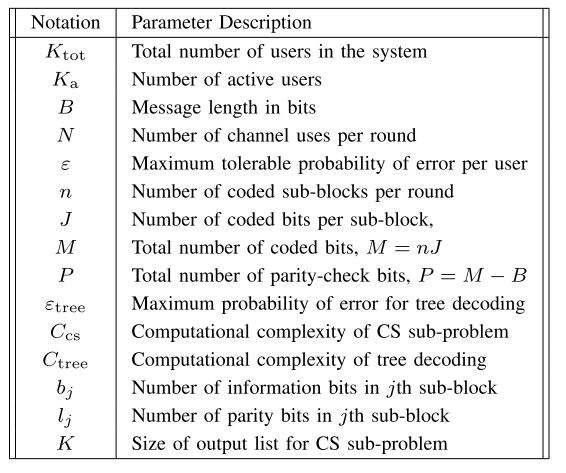
\includegraphics[width=0.45\linewidth]{images_CCS/notation.png}
        \caption{Notation
        \footnote{``A Coded Compressed Sensing Scheme for
Unsourced Multiple Access'' Vamsi K. Amalladinne IEEE TIT 2020}
}
        \label{fig:dataset}
    \end{figure}
\vspace{-1em}
 
\end{frame}


\begin{frame}{Big Picture} 
 
    \begin{figure}
        \centering
        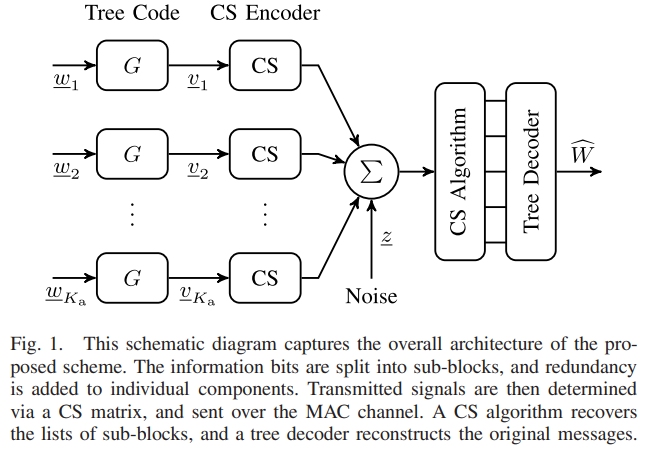
\includegraphics[width=0.6\linewidth]{images_CCS/fig1.png}
        \caption{Architechture\footnote{``A Coded Compressed Sensing Scheme for
Unsourced Multiple Access'' Vamsi K. Amalladinne IEEE TIT 2020}}
        \label{fig:dataset}
    \end{figure}
    
\vspace{-1em}
 
\end{frame}

% \begin{frame}{Encoding}
%     \begin{figure}
%         \begin{minipage}[]{0.5\linewidth}
%             % Left side for text
%             \begin{itemize}
%                 \item 
%                 \begin{equation*}
%                     \underline{p}(j)=\sum_{\ell=0}^{j-1}\underline{w}(\ell)G_{\ell,j-1}
%                 \end{equation*}
%             \end{itemize}
%         \end{minipage}%
%         \begin{minipage}[t]{0.5\linewidth}
%             % Right side for figure
%             \centering
%             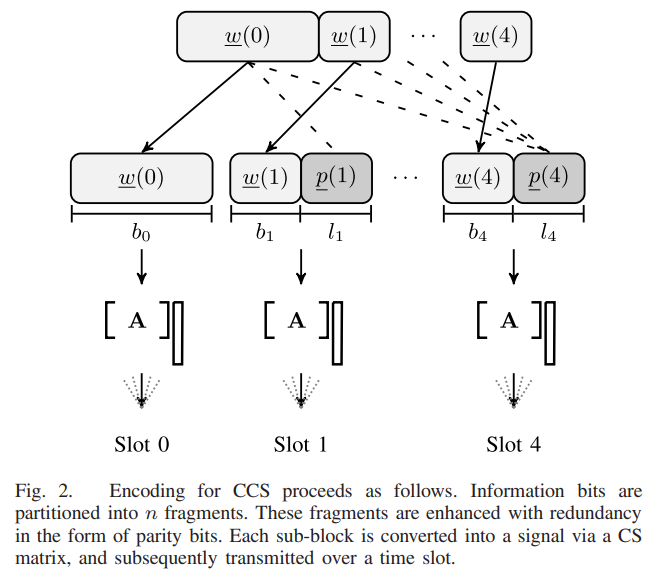
\includegraphics[width=\linewidth]{images_CCS/fig2.png}
%             \caption{Notation}
%             \label{fig:dataset}
%         \end{minipage}
%     \end{figure}
% \end{frame}
\begin{frame}{Encoding}
    \begin{figure}
        \begin{minipage}{0.5\linewidth}
            % Left side for text
            \begin{itemize}
                \item Tree Encoding
                \begin{equation*}
                    \underline{p}(j)=\sum_{\ell=0}^{j-1}\underline{w}(\ell)G_{\ell,j-1}
                \end{equation*}
               
                \begin{equation*}
                    \underline{v}=\underbrace{\underline{w}(0)}_{\underline{v}(0)}\underbrace{\underline{w}(1)\underline{p}(1)}_{\underline{v}(1)}\cdots\underbrace{\underline{w}(n-1)\underline{p}(n-1)}_{\underline{v}(n-1)}.
                \end{equation*}
                \item CS Encoding 
            \end{itemize}
        \end{minipage}%
        \begin{minipage}{0.5\linewidth}
            % Right side for figure
            \centering
            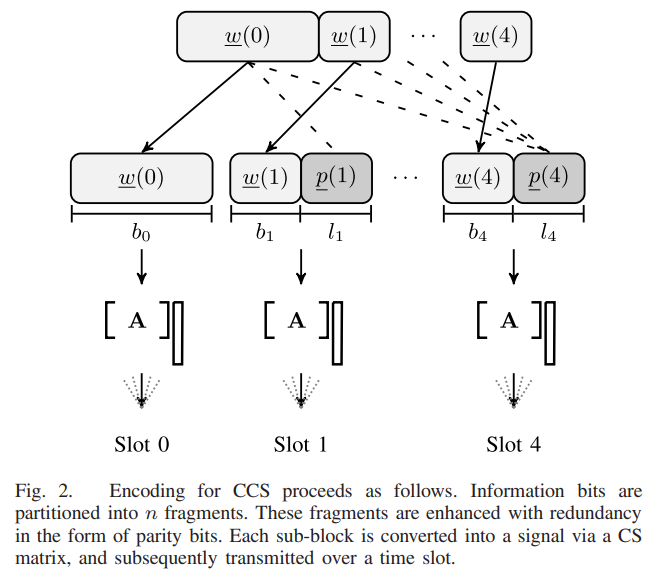
\includegraphics[width=\linewidth]{images_CCS/fig2.png}
            \caption{Encoding\footnote{``A Coded Compressed Sensing Scheme for
Unsourced Multiple Access'' Vamsi K. Amalladinne IEEE TIT 2020}}
            \label{fig:dataset}
        \end{minipage}
    \end{figure}
\end{frame}
\section{Dive in Details}
\subsection{Encoding}
\begin{frame}{Tree Encoding}{Optimization Framework}
    \begin{columns}
        \begin{column}{0.5\textwidth}
            % Left side content
           \begin{itemize}
               \item B-bit binary message partitioned into $n$ sub-blocks, where the $j$th sub-block consisting of $b_{j}$ message bits, with$\sum _{j= 0}^{n- 1}b_{j}= B.$
               \item $\underline {w}= \underline {w}( 0) \underline {w}( 1) \cdots \underline {w}( n- 1) .$ 
               \item The tree encoder appends $l_j$ parity check bits to sub-block $j$,   total length of every sub-block to $b_j+l_j=J=$ $M/\bar{n \hspace{0.1cm}bits
              }$
               \item $  b_0=J$   $l_0=0$   For subsequent subblocks, the parity bits are constructed as follows. 
                         \begin{equation*}
                    \underline{p}(j)=\sum_{\ell=0}^{j-1}\underline{w}(\ell)G_{\ell,j-1}
                \end{equation*}
               
           \end{itemize}
        \end{column}
        \begin{column}{0.5\textwidth}
            % Right side content
            \begin{aligned}
& \\
&\min_{(p_1,\ldots,p_{n-1})}&& \mathbb{E}[\tilde{C}_{\mathrm{tree}}]  \\
&\text{subject to}&& \mathbb{E}\big[\tilde{L}_{n-1}\big]\leq\varepsilon_{\mathrm{tree}}  \\
&&&\sum_{j=1}^{n-1}\log_{2}\left(\frac{1}{p_{j}}\right)=M-B \\
&&&p_{j}\in\left[{\frac{1}{2^{J}}},1\right]\quad\forall j\in[1:n-1].


\end{aligned}
$p_{\ell}=2^{-l_{\ell}}.$
        \end{column}
    \end{columns}
\end{frame}

\subsection{Decoding} 
\begin{frame}{Decoding}{CS Decoding}
    \begin{figure}
        \begin{minipage}{0.5\linewidth}
            % Left side for text
            \begin{itemize}
                \item 
                The aggregate signal received at the base station during the $j$th sub-block can be expressed as $y(j)=$ $\mathbf{A}r(j)+z(j)$, where $r(j) $ is a $K_\text{a}-$sparse binary
                
                
            \end{itemize}
        \end{minipage}%
        \begin{minipage}{0.5\linewidth}
            % Right side for figure
            \centering
            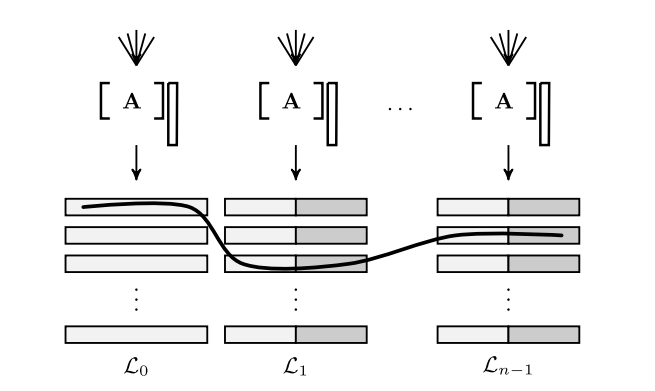
\includegraphics[width=\linewidth]{images_CCS/fig3.png}
            \caption{Decoding\footnote{``A Coded Compressed Sensing Scheme for Unsourced Multiple Access'' Vamsi K. Amalladinne IEEE TIT 2020}}
            \label{fig:dataset}
        \end{minipage}
    \end{figure}
\end{frame}
 

 
\begin{frame}{Tree Decoding}
    \begin{figure}
        \centering
        \begin{minipage}[b]{0.4\linewidth}
            \centering
            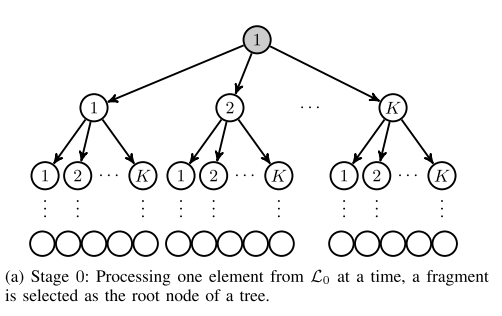
\includegraphics[width=\linewidth]{images_CCS/fig4a.png}
            % \caption{Caption for Figure 1}
            \label{fig:fig1}
        \end{minipage}
        \hfill
        \begin{minipage}[b]{0.4\linewidth}
            \centering
            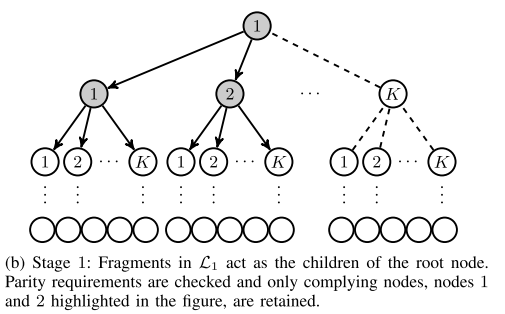
\includegraphics[width=\linewidth]{images_CCS/fig4b.png}
            % \caption{Caption for Figure 2}
            \label{fig:fig2}
        \end{minipage}
    \end{figure}
    
    \begin{figure}
        \centering
        \begin{minipage}[b]{0.4\linewidth}
            \centering
            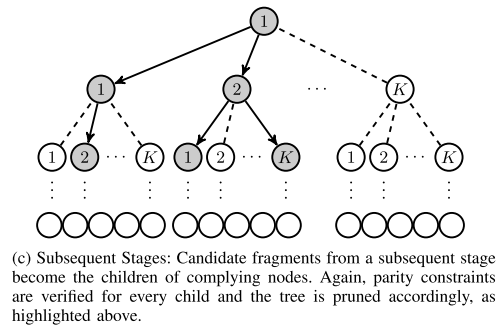
\includegraphics[width=\linewidth]{images_CCS/fig4c.png}
            % \caption{Caption for Figure 3}
            \label{fig:fig3}
        \end{minipage}
        \hfill
        \begin{minipage}[b]{0.4\linewidth}
            \centering
            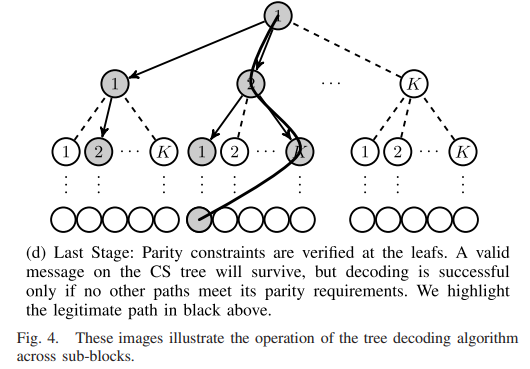
\includegraphics[width=\linewidth]{images_CCS/fig4d.png}
            % \caption{Caption for Figure 4}
            \label{fig:fig4}
        \end{minipage}
    \end{figure}
\end{frame}
\section{Implementation}
\begin{frame}{Implementation Details}
    \begin{itemize}
        \item Message Generation - Selection of Data Structures
        \item Tree Encoding - Optimisation of parity-bits length using \texttt{CVXPY} framwork
        \item CS Encoding - Sensing Matrix generation using BCH codes
        \item CS Decoding - Orthogonal Matching Pursuit
        \item Tree Decoding - Backtracking with pruning
    \end{itemize}
\end{frame}
\begin{frame}{Simulation Details}
    \begin{itemize}
        \item According to the reference
        \item $K_a=25$
        \item $B = 101$
        \item $n = 11$
        \item $J = 15$
        \item $\varepsilon_\text{tree}=0.0025$
        \item $(2047,23)$ BCH Codebook
    \end{itemize}
\end{frame}

\begin{frame}{Challenges}
\begin{itemize}
    \item Infeasibility of the parity length optimisation for some $varepsilon_\text{tree}$
    \item Failure of the total bits constraint due to rounding of parity lengths
    \item Vectorisation of the otherwise inefficient tree encoding code
    \item Edge cases in tree decoding due to missing data
    \item Slowed working of CS decoding for higher $J$
    
\end{itemize}
\end{frame}

\begin{frame}{Results}{Optimization Framework}
\begin{table}[h]
\centering
\begin{tabular}{|c|c|c|}
\hline
$\varepsilon_{\mathrm{tree}}$ & $\mathrm{E}[\bar{C}_{\mathrm{tree}}]$ & \text{Parity Length Vector} \\
\hline
0.0001 & \multicolumn{2}{c|}{Infeasible} \\
0.001 & 555 & 0 4 5 5 5 5 5 5 6 8 16 \\
0.0012 & 516 & 0 4 5 5 5 5 5 6 6 7 16 \\
0.0015 & 493 & 0 3 5 5 6 6 6 6 6 6 15 \\
0.0020 & 477 & 0 4 5 5 5 6 6 6 6 6 15 \\
0.0025 & 466 & 0 4 5 5 6 6 6 6 6 6 14 \\
0.006 & 429 & 0 4 5 6 6 6 6 6 6 6 13 \\
0.008 & 419 & 0 4 6 6 6 6 6 6 6 6 12 \\
0.02 &  392 & 0 5 6 6 6 6 6 6 6 6 11 \\
\hline
\end{tabular}
\caption{Error Probability is minimized when Parity Check Bits are Pushed to End, whereas\\ Average Computational Complexity is Least when equal parity-check bits are allocated per sub-block}
\label{tab:my_table}
\end{table}

\end{frame}

\begin{frame}{Results}{Simulation}
For the mentioned parameter set,
    \begin{itemize}
        \item Complete recovery of messages wasn't possible
        \item 30\%-40\% of bits recovered partially
        \item Hence efficient Code design at client level needed
    \end{itemize}
    \begin{figure}
        \centering
        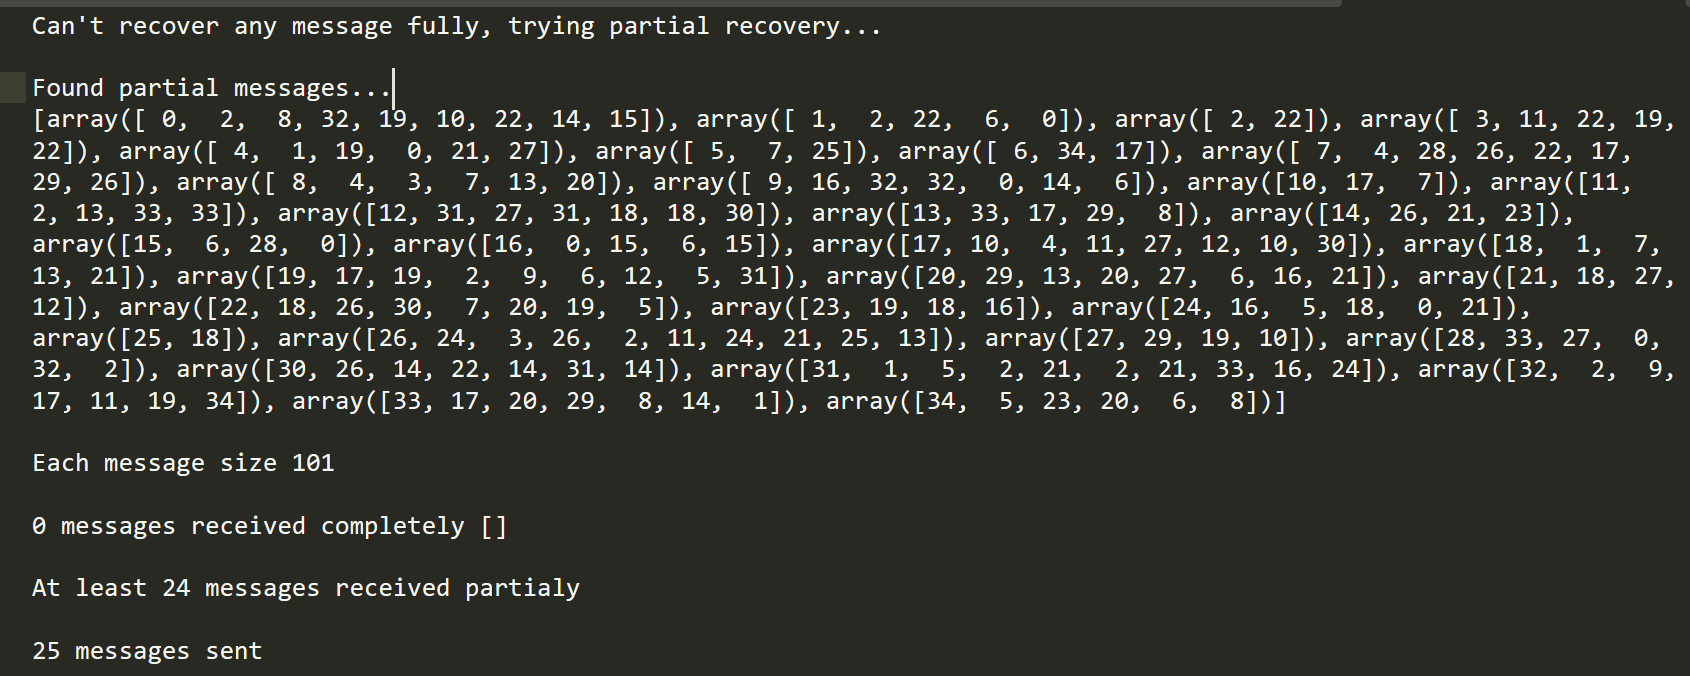
\includegraphics[width=0.8\linewidth]{images_CCS/results.png}
    \end{figure}
\end{frame}


 \begin{frame}{Future Work}
     \begin{itemize}
         \item Detailed analysis of the algorithm for varying \#users with a better metric such as $E_b/N_0$
         \item Comparison with other state-of-the-art techniques such as ALOHA and SIC
         \item Hyperparameter tuning to obtain optimal results
     \end{itemize}
 \end{frame}

% \subsection{Dataset}
% \begin{frame}{Dataset}{Columbia University Image Library
% (COIL-100)}
% 100 objects! Each object has 72 pose images with pose angle $\{0,5,10,\ldots,345,350,355\}$
%     \begin{figure}
%         \centering
%         \includegraphics[width=0.45\linewidth]{Sample-images-from-COIL-100-database.jpg}
%         \caption{COIL-100 Dataset by Columbia Imaging and Vision Laboratory (CAVE)\footnote{``Columbia Object Image Library,''
% S. A. Nene, S. K. Nayar and H. Murase, CUCS-006-96, February 1996.}}
%         \label{fig:dataset}
%     \end{figure}
% \vspace{-1em}
% These objects can be categorised into two sets
% \begin{itemize}
%     \item uniform reflectance but similar shape
%     \item complex reflectance and geometric properties
% \end{itemize}
% \end{frame}

% \begin{frame}{Equations} 
    
%     \begin{itemize}
%         \item Image Assumptions
       
%     \end{itemize}
% \end{frame}

% \begin{frame}{Manifold (Parametric Appearance Representation)}{Examples}
%     \begin{figure}
%         \centering
%         \begin{subfigure}{0.32\linewidth}
%             \centering
%             \includegraphics[width = 0.6\linewidth]{splines/obj3__0.png}
%             \vspace{1em}
%             \caption{Object 2}
%         \end{subfigure}
%         \begin{subfigure}{0.32\linewidth}
%             \centering
%             \includegraphics[width = 0.6\linewidth]{splines/obj4__0.png}
%             \vspace{1em}
%             \caption{Object 3}
%         \end{subfigure}
%         \begin{subfigure}{0.32\linewidth}
%             \centering
%             \includegraphics[width = 0.6\linewidth]{splines/obj5__0.png}
%             \vspace{1em}
%             \caption{Object 4}
%         \end{subfigure}
%         \begin{subfigure}{0.32\linewidth}
%             \centering
%             \includegraphics[width = \linewidth]{splines/2.pdf}
%             \caption{Corresponding Manifold}
%         \end{subfigure}
%         \begin{subfigure}{0.32\linewidth}
%             \centering
%             \includegraphics[width = \linewidth]{splines/3.pdf}
%             \caption{Corresponding Manifold}
%         \end{subfigure}
%         \begin{subfigure}{0.32\linewidth}
%             \centering
%             \includegraphics[width = \linewidth]{splines/4.pdf}
%             \caption{Corresponding Manifold}
%         \end{subfigure}
%     \end{figure}
% \end{frame}
% \subsection{Code Optimizations}
% \begin{frame}[fragile]{Code Optimizations}{Implementation}
%     \begin{itemize}
%         \item Principal Component Analysis (PCA)
%         \begin{itemize}
%             \item Eigenvector computation of $X^TX$ instead of the covariance matrix ($XX^T$)
%             \item \verb!numpy.linalg.eigh! instead to \verb!numpy.linalg.eig! to exploit the algorithms assuming symmetric input matrices
%         \end{itemize}
%         \item Extensive usage of \verb!numpy! objects and functions to facilitate multi-threading in \verb!numba!
%         \item \verb!os.environ[`OMP_NUM_THREADS'] = `16'! to increase number of parallel threads to 16
%         \item Ability to store and load saved learnt variables using \verb!pickle!
%     \end{itemize}
% \end{frame}
% \section{Results and Observations}
% \subsection{Optimal PCA Threshold and Training Data Split}
% \subsection{Variation with PCA Threshold and Training Data Split one at a time}
% \begin{frame}{Optimal Values}{PCA Threshold = 0.6 and Training Data Split = 0.7}
%     \begin{description}
%         \item[Object Recognition accuracy]  99.172\%
%         \item[Pose Estimation accuracy] 76.172\%
%         \item[Mean Pose error] 6.872$^\circ$
%     \end{description}
%     In the next two slides, we see some examples of incorrect recognition. 
    
%     Even in such cases we see that our model's outputs are reasonable.
%     \begin{itemize}
%         \item 180$^\circ$ pose errors are most frequent among pose recognition
%         \item similar-looking objects get recognised incorrectly
%     \end{itemize}
%     These errors usually occur in bursts (consecutive poses), which implies that nearby points in manifolds might be too far to interpolate in between points accurately.
    
%     One way to solve this is by training on uniformly pose-separated object images.
    
% \end{frame}
% \subsection{Incorrect Object Detection}
% \begin{frame}{Incorrect Object Detection (True and Estimated)}
%     \begin{figure}
%         \centering
%         % \begin{subfigure}{0.32\linewidth}
%         %     \centering
%         %     \includegraphics[width = 0.6\linewidth]{incorrect/obj23__90.png}
%         %     \vspace{1em}
%         %     \caption{Obect 22, Angle 90}
%         % \end{subfigure}
%         \begin{subfigure}{0.32\linewidth}
%             \centering
%             \includegraphics[width = 0.6\linewidth]{incorrect/obj8__75.png}
%             \vspace{1em}
%             \caption{Obect 7, Angle 75}
%         \end{subfigure}
%         \begin{subfigure}{0.32\linewidth}
%             \centering
%             \includegraphics[width = 0.6\linewidth]{incorrect/obj23__280.png}
%             \vspace{1em}
%             \caption{Obect 22, Angle 280}
%         \end{subfigure}
%         \begin{subfigure}{0.32\linewidth}
%             \centering
%             \includegraphics[width = 0.6\linewidth]{incorrect/obj98__195.png}
%             \vspace{1em}
%             \caption{Obect 97, Angle 195}
%         \end{subfigure}
%         % \begin{subfigure}{0.32\linewidth}
%         %     \centering
%         %     \includegraphics[width = 0.6\linewidth]{incorrect/obj78__90.png}
%         %     \vspace{1em}
%         %     \caption{Object 77, Angle 90}
%         % \end{subfigure}
%         \begin{subfigure}{0.32\linewidth}
%             \centering
%             \includegraphics[width = 0.6\linewidth]{incorrect/obj23__80.png}
%             \vspace{1em}
%             \caption{Object 22, Angle 80}
%         \end{subfigure}
%         \begin{subfigure}{0.32\linewidth}
%             \centering
%             \includegraphics[width = 0.6\linewidth]{incorrect/obj76__280.png}
%             \vspace{1em}
%             \caption{Object 75, Angle 280}
%         \end{subfigure}
%         \begin{subfigure}{0.32\linewidth}
%             \centering
%             \includegraphics[width = 0.6\linewidth]{incorrect/obj84__25.png}
%             \vspace{1em}
%             \caption{Object 83, Angle 25}
%         \end{subfigure}
%     \end{figure}
% \end{frame}
% \begin{frame}{Incorrect Pose Recognition (True and Estimated)}
%     \begin{figure}
%         \centering
%         \begin{subfigure}{0.32\linewidth}
%             \centering
%             \includegraphics[width = 0.6\linewidth]{incorrect/obj34__75.png}
%             \vspace{1em}
%             \caption{Obect 33, Angle 75}
%         \end{subfigure}
%         \begin{subfigure}{0.32\linewidth}
%             \centering
%             \includegraphics[width = 0.6\linewidth]{incorrect/obj22__280.png}
%             \vspace{1em}
%             \caption{Obect 21, Angle 280}
%         \end{subfigure}
%         \begin{subfigure}{0.32\linewidth}
%             \centering
%             \includegraphics[width = 0.6\linewidth]{incorrect/obj21__100.png}
%             \vspace{1em}
%             \caption{Obect 20, Angle 100}
%         \end{subfigure}
%         \begin{subfigure}{0.32\linewidth}
%             \centering
%             \includegraphics[width = 0.6\linewidth]{incorrect/obj34__80.png}
%             \vspace{1em}
%             \caption{Object 33, Angle 80}
%         \end{subfigure}
%         \begin{subfigure}{0.32\linewidth}
%             \centering
%             \includegraphics[width = 0.6\linewidth]{incorrect/obj22__95.png}
%             \vspace{1em}
%             \caption{Object 21, Angle 95}
%         \end{subfigure}
%         \begin{subfigure}{0.32\linewidth}
%             \centering
%             \includegraphics[width = 0.6\linewidth]{incorrect/obj21__280.png}
%             \vspace{1em}
%             \caption{Object 20, Angle 280}
%         \end{subfigure}
%     \end{figure}
% \end{frame}
% \begin{frame}{Variation with PCA Threshold and Training Data Split one at a time}
%     In the coming plots, we vary each parameter one by one and then vary them simultaneously
%     \begin{itemize}
%         \item Vary PCA Threshold as $\{0.05, 0.1,\ldots, 0.9, 0.95\}$, set Training Data Split to 0.6
%         \begin{itemize}
%             \item higher PCA Threshold leads to overfitting 
%         \end{itemize}
%         \item Vary Training Data Split as $\{0.05, 0.1,\ldots, 0.9, 0.95\}$, set PCA Threshold to 0.7
%         \begin{itemize}
%             \item more training data creates more accurate manifold which leads to better recognition
%         \end{itemize}
%         \item Vary PCA Threshold as $\{0.05, 0.1,\ldots, 0.9, 0.95\}$ and 
        
%         vary Training Data Split as $\{0.05, 0.1,\ldots, 0.9, 0.95\}$
%     \end{itemize}
% \end{frame}
% \begin{frame}{Variation with PCA Threshold and Training Data Split one at a time}{Accuracy}
%     \begin{figure}
%         \centering
%         \begin{subfigure}{0.48\linewidth}
%             \centering
%             \includegraphics[width=\linewidth]{pca/accuracy_overall.pdf}
%         \end{subfigure}
%         \begin{subfigure}{0.48\linewidth}
%             \centering
%             \includegraphics[width=\linewidth]{tds/accuracy_overall.pdf}
%         \end{subfigure}
%     \end{figure}
% \end{frame}
% \begin{frame}{Variation with PCA Threshold and Training Data Split one at a time}{Mean Error}
%     \begin{figure}
%         \centering
%         \begin{subfigure}{0.48\linewidth}
%             \centering
%             \includegraphics[width=\linewidth]{pca/mean_error_overall.pdf}
%         \end{subfigure}
%         \begin{subfigure}{0.48\linewidth}
%             \centering
%             \includegraphics[width=\linewidth]{tds/mean_error_overall.pdf}
%         \end{subfigure}
%     \end{figure}
% \end{frame}
% \begin{frame}{Variation with PCA Threshold and Training Data Split one at a time}{Object Accuracy}
%     \begin{figure}
%         \centering
%         \begin{subfigure}{0.48\linewidth}
%             \centering
%             \includegraphics[width=\linewidth]{pca/object_accuracy_all_objects.pdf}
%         \end{subfigure}
%         \begin{subfigure}{0.48\linewidth}
%             \centering
%             \includegraphics[width=\linewidth]{tds/object_accuracy_all_objects.pdf}
%         \end{subfigure}
%     \end{figure}
% \end{frame}
% \begin{frame}{Variation with PCA Threshold and Training Data Split one at a time}{Pose Accuracy}
%     \begin{figure}
%         \centering
%         \begin{subfigure}{0.48\linewidth}
%             \centering
%             \includegraphics[width=\linewidth]{pca/pose_accuracy_all_objects.pdf}
%         \end{subfigure}
%         \begin{subfigure}{0.48\linewidth}
%             \centering
%             \includegraphics[width=\linewidth]{tds/pose_accuracy_all_objects.pdf}
%         \end{subfigure}
%     \end{figure}
% \end{frame}
% \begin{frame}{Variation with PCA Threshold and Training Data Split one at a time}{Mean Error}
%     \begin{figure}
%         \centering
%         \begin{subfigure}{0.48\linewidth}
%             \centering
%             \includegraphics[width=\linewidth]{pca/mean_error_all_objects.pdf}
%         \end{subfigure}
%         \begin{subfigure}{0.48\linewidth}
%             \centering
%             \includegraphics[width=\linewidth]{tds/mean_error_all_objects.pdf}
%         \end{subfigure}
%     \end{figure}
% \end{frame}
% \begin{frame}{Variation with PCA Threshold and Training Data Split one at a time}{Exact Error}
%     \begin{figure}
%         \centering
%         \begin{subfigure}{0.48\linewidth}
%             \centering
%             \includegraphics[width=\linewidth]{pca/error_histogram_overall.pdf}
%         \end{subfigure}
%         \begin{subfigure}{0.48\linewidth}
%             \centering
%             \includegraphics[width=\linewidth]{tds/error_histogram_overall.pdf}
%         \end{subfigure}
%     \end{figure}
% \end{frame}
% \subsection{Simultaneous variation with PCA Threshold and Training Data Split}
% \begin{frame}{Simultaneous variation with PCA Threshold and Training Data Split}
%     \begin{figure}
%         \centering
%         \begin{subfigure}{0.32\linewidth}
%             \centering
%             \includegraphics[width=\linewidth]{combined/object_accuracy_overall.pdf}
%             \caption{Object Accuracy}
%         \end{subfigure}
%         \begin{subfigure}{0.32\linewidth}
%             \centering
%             \includegraphics[width=\linewidth]{combined/pose_accuracy_overall.pdf}
%             \caption{Pose Accuracy}
%         \end{subfigure}
%         \begin{subfigure}{0.32\linewidth}
%             \centering
%             \includegraphics[width=\linewidth]{combined/mean_error_overall.pdf}
%             \caption{Mean Error}
%         \end{subfigure}
%     \end{figure}
% \end{frame}
% \subsection{Observations (Three types of objects)}
% \begin{frame}{Observations}{Three types of objects}
% % \begin{enumerate}[(a)]
% \begin{itemize}
%     \item Simple Objects, almost no variation in poses due to symmetrical nature and less details
%     \item Simple Objects, almost no variation in poses due to symmetrical nature but highly detailed
%     \item Complex Objects, different shapes in different poses
% \end{itemize}
% % \end{enumerate}
%     \begin{figure}
%         \centering
%         \begin{subfigure}{0.32\linewidth}
%             \centering
%             \includegraphics[width = 0.6\linewidth]{wireframe/obj70__0.png}
%             \vspace{1em}
%             \caption{Object 69}
%         \end{subfigure}
%         \begin{subfigure}{0.32\linewidth}
%             \centering
%             \includegraphics[width = 0.6\linewidth]{wireframe/obj99__0.png}
%             \vspace{1em}
%             \caption{Object 98}
%         \end{subfigure}
%         \begin{subfigure}{0.32\linewidth}
%             \centering
%             \includegraphics[width = 0.6\linewidth]{wireframe/obj68__0.png}
%             \vspace{1em}
%             \caption{Object 67}
%         \end{subfigure}
%     \end{figure}
% \end{frame}
% \begin{frame}{Observations}{Types of Wireframe: Mean Accuracy}
% \begin{itemize}
%     \item as object complexity increases, more training data is needed for lower mean error
%     \item only slightly higher pca threshold needed for complex objects
% \end{itemize}
%     \begin{figure}
%         \centering
%         \begin{subfigure}{0.32\linewidth}
%             \centering
%             \includegraphics[width=1.2\linewidth]{wireframe/error/69.pdf}
%             \caption{Object 69}
%         \end{subfigure}
%         \begin{subfigure}{0.32\linewidth}
%             \centering
%             \includegraphics[width=1.2\linewidth]{wireframe/error/98.pdf}
%             \caption{Object 98}
%         \end{subfigure}
%         \begin{subfigure}{0.32\linewidth}
%             \centering
%             \includegraphics[width=1.2\linewidth]{wireframe/error/67.pdf}
%             \caption{Object 67}
%         \end{subfigure}
        
%     \end{figure}
% \end{frame}
% \begin{frame}{Observations}{Types of Wireframe: Object Accuracy}
% \begin{itemize}
%     \item as object complexity increases, more training data is needed for higher accuracy

%     15-20 objects poses are enough for learning the simple objects, but 30-40 object poses are needed to learn complex dataset
%     \item higher pca threshold only needed in complex objects
% \end{itemize}
%     \begin{figure}
%         \centering
%         \begin{subfigure}{0.32\linewidth}
%             \centering
%             \includegraphics[width=1.2\linewidth]{wireframe/object/69.pdf}
%             \caption{Object 69}
%         \end{subfigure}
%         \begin{subfigure}{0.32\linewidth}
%             \centering
%             \includegraphics[width=1.2\linewidth]{wireframe/object/98.pdf}
%             \caption{Object 98}
%         \end{subfigure}
%         \begin{subfigure}{0.32\linewidth}
%             \centering
%             \includegraphics[width=1.2\linewidth]{wireframe/object/67.pdf}
%             \caption{Object 67}
%         \end{subfigure}
%     \end{figure}
% \end{frame}
% \begin{frame}{Observations}{Types of Wireframe: Pose Accuracy}
% \begin{itemize}
%     \item accuracy increases as object complexity increases, because pose becomes easier to distinguish
%     \item for simpler objects, more training data or pca threshold doesn't help much to estimate exactly
% \end{itemize}
%     \begin{figure}
%         \centering
%         \begin{subfigure}{0.32\linewidth}
%             \centering
%             \includegraphics[width=1.2\linewidth]{wireframe/pose/69.pdf}
%             \caption{Object 69}
%         \end{subfigure}
%         \begin{subfigure}{0.32\linewidth}
%             \centering
%             \includegraphics[width=1.2\linewidth]{wireframe/pose/98.pdf}
%             \caption{Object 98}
%         \end{subfigure}
%         \begin{subfigure}{0.32\linewidth}
%             \centering
%             \includegraphics[width=1.2\linewidth]{wireframe/pose/67.pdf}
%             \caption{Object 67}
%         \end{subfigure}
%     \end{figure}
% \end{frame}

% \section{Theory (optional)}
% \begin{frame}[allowframebreaks]{Theory}{Notation}
% Single image (normalised)
% \begin{equation}
%             \hat{\mathbf{x}} = 
%         \begin{bmatrix}
%         \hat{x_1}, & \hat{x_2}, & \cdots, & \hat{x_N}
%         \end{bmatrix}^T
%     \end{equation}
% Universal Image Set
%     % \begin{align}
%     %     \mathbf{X} = 
%     %     \{ &\hat{\mathbf{x}}^{(1)}_{1}, \dots, \hat{\mathbf{x}}^{(1)}_{R},\nonumber\\
%     %     &\hat{\mathbf{x}}^{(2)}_{1}, \dots, \hat{\mathbf{x}}^{(2)}_{R},\\
%     %     &\qquad\vdots\nonumber \\
%     %     & \hat{\mathbf{x}}^{(P)}_{1}, \dots,
%     %     \hat{\mathbf{x}}^{(P)}_{R}\} \nonumber
%     % \end{align}
%     % \begin{equation}
%     %     \mathbf{x} = 
%     %     \begin{bmatrix}
%     %     x_1, & x_2, & \cdots, & x_N
%     %     \end{bmatrix}^T
%     % \end{equation}
    
%     % \begin{align}
%     %     x_n = \dfrac{1}{A}\hat{x}_n && A = \sqrt{\sum\limits_{n = 1}^N \hat{x}_n^2}
%     % \end{align}
%     \begin{equation}
%         \mathbf{X} \triangleq \{ \mathbf{x}^{(1)}_{1} - \mathbf{c}, \mathbf{x}^{(1)}_{2} - \mathbf{c}, \dots, \mathbf{x}^{(1)}_{R} - \mathbf{c}, \dots, \mathbf{x}^{(p)}_{R} - \mathbf{c}\}
%     \end{equation}
% Object Image Sets
%     \begin{equation}
%         \mathbf{X}^{(p)} = \{ \hat{\mathbf{x}}^{(p)}_{1} - \mathbf{c}^{(p)}, \hat{\mathbf{x}}^{(p)}_{2} - \mathbf{c}^{(p)}, \dots, \hat{\mathbf{x}}^{(p)}_{R} -  \mathbf{c}^{(p)}\}
%     \end{equation}
% Compute Universal Eigenspace
%     \begin{equation}
%        \mathbf{\hat{Q}} \triangleq \mathbf{X}^T\mathbf{X}
%     \end{equation}

%     \begin{equation}
%         \lambda_i \mathbf{\hat{e}}_i = \mathbf{\hat{Q}}\mathbf{e}_i
%     \end{equation}
% Utilise PCA Threshold $(T_i)$
%     \begin{equation}
%         \dfrac{\sum_{i = 1}^{k} \lambda_i}{\sum_{i = 1}^{N} \lambda_i} \geq T_i
%     \end{equation}
%     \begin{equation}
%         \mathbf{Q} = \mathbf{X}\begin{bmatrix}
%             \mathbf{\hat{e}}_1, & \mathbf{\hat{e}}_2, & \dots & \mathbf{\hat{e}}_{k}
%         \end{bmatrix}
%     \end{equation}
% Similarly, Compute Object Eigenspaces
% \begin{equation}
%        \mathbf{\hat{Q}}^{(p)} \triangleq {\mathbf{X}^{(p)}}^T\mathbf{X}^{(p)}
%     \end{equation}

%     \begin{equation}
%         \lambda_i^{(p)} \mathbf{\hat{e}}_i^{(p)} = \mathbf{\hat{Q}}^{(p)}\mathbf{\hat{e}}_i^{(p)}
%     \end{equation}
% Utilise PCA Threshold $(T_i)$
%     \begin{equation}
%         \dfrac{\sum_{i = 1}^{{k}^{(p)}} \lambda_i^{(p)}}{\sum_{i = 1}^{N} \lambda_i^{(p)}} \geq T_i
%     \end{equation}
%     \begin{equation}
%         \mathbf{Q}^{(p)} = \mathbf{X}^{(p)}\begin{bmatrix}
%             \mathbf{\hat{e}}_1^{(p)}, & \mathbf{\hat{e}}_2^{(p)}, & \dots & \mathbf{\hat{e}}_{k^{(p)}}
%         \end{bmatrix}
%     \end{equation}
% Compute manifolds
%     \begin{equation}
%         \mathbf{g}_{i}^{(p)} =
%         \mathbf{Q}^T
%         (\mathbf{x}_{i}^{(p)} - \mathbf{c})
%     \end{equation}

%     \begin{equation}
%         \mathbf{f}_{i}^{(p)} = 
%         {\mathbf{Q}^{(p)}}^T(\mathbf{x}^{(p)}_{i} - \mathbf{c}^{(p)})
%     \end{equation}
% Interpolate manifolds

% Universal Manifolds
%     \begin{equation}
%         \mathbf{g}^{(p)}(\theta)
% \end{equation}
% Object-specific Manifolds    
%     \begin{equation}
%         \mathbf{f}^{(p)}(\theta)
% \end{equation}
% % Given image $\mathbf{y}$ projected to eigenspace
% Closest universal manifold from projection of given image $\mathbf{y}$
%   \begin{equation}
%      \mathbf{z} = 
%         \mathbf{Q}^T
%         (\mathbf{y} - \mathbf{c})
%     \end{equation}
%     \begin{equation}
%         d_1^{(p)} = \min_{\theta} \| \mathbf{z} - \mathbf{g}^{p}(\theta) \|
%     \end{equation}
% Point on object manifold closest from project of given image $\mathbf{y}$
%     \begin{equation}
%      \mathbf{z}^{(p)} = 
%         {\mathbf{Q}^{(p)}}^T
%         (\mathbf{y} - \mathbf{c}^{(p)})
%     \end{equation}
%     \begin{equation}
%         d_2^{(p)} = \min_{\theta} \| \mathbf{z}^{(p)} - \mathbf{f}^{p}(\theta) \|
%     \end{equation}
% \end{frame}

% \appendix


\section{References}
\begin{frame}%[allowframebreaks]
  \frametitle<presentation>{References}
%   \bibliographystyle{plainnat}    
\bibliographystyle{plainurl}
  \nocite{*}
  {\bibliography{references}}
%   \begin{thebibliography}{10}
    
%   \beamertemplatebookbibitems
%   % Start with overview books.

%   \bibitem{Author1990}
%     A.~Author.
%     \newblock {\em Handbook of Everything}.
%     \newblock Some Press, 1990.
 
    
%   \beamertemplatearticlebibitems
%   % Followed by interesting articles. Keep the list short. 

%   \bibitem{Someone2000}
%     S.~Someone.
%     \newblock On this and that.
%     \newblock {\em Journal of This and That}, 2(1):50--100,
%     2000.
%   \end{thebibliography}
\end{frame}

\begin{frame}{Contribution}
    \begin{itemize}
        \item Param: Decoder, Message Generation, overall code maintainence with vectorisation
        \item Satush: Encoder, Parity Length Optimisation, Sensing Matrix Generation
    \end{itemize}
\end{frame}



\end{document}